
%Blockschaltbild Phasenschieberoszillator 
\documentclass{article}
\usepackage{tikz}
\usetikzlibrary{shapes.geometric, arrows, positioning}

\begin{document}

\begin{figure}
  \centering
  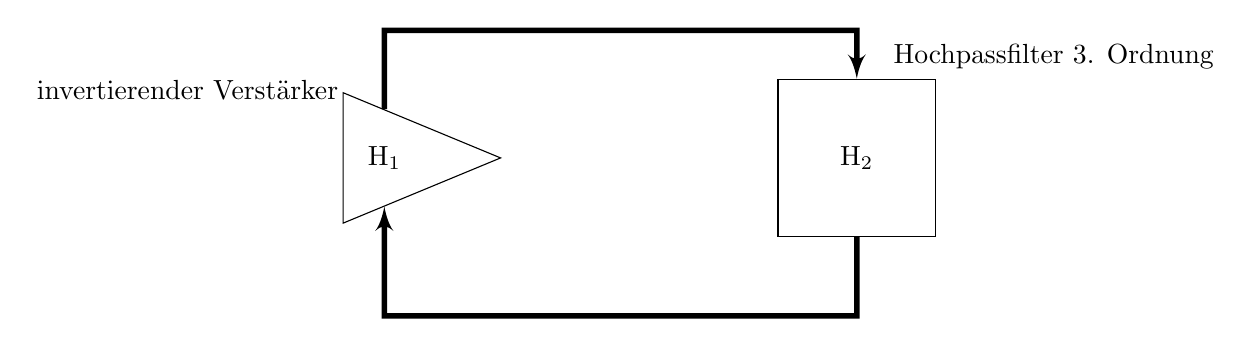
\begin{tikzpicture}[auto, node distance=3.5cm, >=latex']
    % Nodes
    \node [isosceles triangle, draw, minimum height=2cm, scale=1] (H1) {H$_1$};
    \node [rectangle, draw, right of=H1, node distance=6cm, minimum height=2cm, minimum width=2cm, scale=1] (H2) {H$_2$};
    
    % Texts
    \node [above, xshift=-2.5cm, font=\normalsize] at (H1.north) {invertierender Verstärker};
    \node [above, xshift=2.5cm, font=\normalsize] at (H2.north) {Hochpassfilter 3. Ordnung};
    
    % Arrows
    \draw [->, line width=2pt] (H1.north) -- ++(0,1) -- ++(6,0) -- (H2.north);
    \draw [->, line width=2pt] (H2.south) -- ++(0,-1) -- ++(-6,0) -- (H1.south);

  \end{tikzpicture}

\end{figure}

\end{document}

\begin{tikzpicture}[
        %Global Config
        font=\small
    ]

%You can create an smart objet like Henry Menke in this post http://www.texample.net/tikz/examples/4-bit-counter/
% Variables: 1: Position 2: ID.
 \def\TIMER555(#1)#2{%
  \begin{scope}[shift={(#1)}]
    \draw[fill=blue!10] (-1.5,-2) rectangle (1.5,2); % The body of IC
    % Label and component identifier.
    \draw[red] (2,2.5) node []{\large \bfseries  U - #2}; % IC LABEL
    \draw[red] (0,0.5) node [align=center]{\large NE-555\\TIMER}; % IC LABEL
    % Draw the pins
    % Some that you have to learn about label nodes, draw lines, and name coordinates in Tikz
    \draw (0.9,-2) node [above]{GND} -- +(0,-0.5) node [anchor=-45]{1} coordinate (#2 GND); % Pin 1 GND
    \draw (-1.5,-1.5) node [right]{TRG} -- +(-0.5,0) node [anchor=-135]{2} coordinate (#2 TRG); % Pin 2 TRG
    \draw (1.5,0) node [left]{OUT} -- +(0.5,0) node [anchor=-45]{3} coordinate (#2 OUT); % Pin 3 OUT  
    \draw (0.9,2) node [below]{RESET} -- +(0,0.5) node [anchor=45]{4} coordinate (#2 RESET); % Pin 4 RESET
    \draw (0,-2) node [above]{CTRL} -- +(0,-0.5) node [anchor=-45]{5} coordinate (#2 CTRL); % Pin 5 CTRL
    \draw (-1.5,-.5) node [right]{THR} -- +(-0.5,0) node [anchor=-135]{6} coordinate (#2 THR); % Pin 6 THR
    \draw (-1.5,1.5) node [right]{DIS} -- +(-0.5,0) node [anchor=-135]{7} coordinate (#2 DIS); % Pin 7 DIS
    \draw (0,2) node [below]{$\mathsf{V_{CC}}$} -- +(0,0.5) node [anchor=45]{8} coordinate (#2 VCC); % Pin 8 VCC
  \end{scope}
}

% Start drawing the circuit: Example "Dee-Dah" Siren

% Place the IC's in position
\TIMER555(0,0){1}

%Place polarization nodes:
\draw (-4.5,3.5) node[ocirc] (VCC){} node[left]{$\mathsf{V_{CC}}$};
\draw (-4.5,-4) node[ocirc] (GND){} node[left]{GND};

% Connect U-1
\draw(VCC) % Start point
    to [short, o-] ++(1,0) coordinate (NOD1) % Use auxiliar coordinate (NOD1)
    to [R, l^=R,*-*] (1 DIS -| NOD1) % to the point in the intersection between NOD1 and 1 DIS
    to [eC,l^=C,*-] ++(0,-2)
    to [short] (GND -| NOD1)
    to [short] (GND);

\draw(1 VCC) to [short, -*] (1 VCC |- NOD1);
\draw(1 RESET) to [short] (1 RESET |- NOD1) to [short] (NOD1);
\draw(1 DIS) to [short, -*] (1 DIS -| NOD1);
\draw(1 THR) to [short] ++ (-0.5,0) coordinate (NOD2) to [short,-*] (1 DIS -| NOD2);
\draw(1 CTRL) to [eC,l_=0.01nF, -*] (1 CTRL |- GND);
\draw(1 GND) to [short] (1 GND |- GND) to [short] (GND -| NOD1);

%Place input/output nodes
\draw[color=blue,line width=2] (1 TRG) to [short] ++(-0.55,0) node[ocirc] (TRG){} node[below]{Trigger};
\draw[color=red,line width=2] (1 OUT) to [short] ++(0.55,0) node[ocirc](OUT){} node[below]{Out};



\end{tikzpicture}
%Notizen